
After completing this chapter, you should be able to:

\begin{enumerate}
 \item Explain Hooke's Law in regards to mass-spring systems, where there is an external force. Construct and solve differential equations which represent this physical model, with or without the presence of a damper and be able to interpret how solutions change based on changes in the model. 
 \item Explain how to obtain solutions to non homogeneous ODEs by finding a particular solution $y_p$ and the kernel $y_h$ to the corresponding homogeneous ODE. 
 \item Use the method of undetermined coefficients to solve non homogeneous linear ODEs.
 \item Explain Kirchhoff's voltage law, Ohm's law, and how to model electrical circuits using 2nd order non homogeneous linear ODEs.  Illustrate how results about circuits can be translated into results about mass-spring systems.
\end{enumerate}



\section{Non Homogeneous Linear Systems}
In the previous chapter, we focused on solving homogeneous ODEs of the form $L(y) = 0$. We need to learn how to solve non homogeneous ODEs, namely $L(y) = r(t)$ where $r(t)\neq 0$. Before solving these kinds of ODEs, let's revisit solving matrix equations of the form $A\vec x=\vec 0$ (homogeneous) and $A\vec x = \vec b$ (non homogeneous).  As we compare the solutions to these matrix equations (where solving is much easier), we'll glean some patterns that help us with solving non homogeneous ODEs.


I highly suggest you complete this review problem, and check your answer, to make sure you are comfortable with how to express infinitely many solutions in vector form. 
\begin{review*}
 Suppose we want to solve the system $A\vec x = \vec b$. We row reduce the augmented matrix and obtain
$$
\begin{bmatrix}
A&\vec b
\end{bmatrix}\xrightarrow{rref}
\begin{bmatrix}
1&0&-3&4&0&5\\
0&1&2&1&0&-2\\
0&0&0&0&1&3\\
0&0&0&0&0&0
\end{bmatrix}.
$$
What's the solution? Give a basis for the kernel of $A$? See \footnote{
The free variables are $x_3$ and $x_4$, as these columns don't have a pivot). The three nonzero rows of our rref give the equations
$x_1-3x_3+4x_4=5$,
$x_2+2x_3+x_4=-2$, and 
$x_5=3$. We solve for each variable in terms of the free variables to obtain
\begin{center}
\begin{tabular}{ccc}
$\begin{array}{l}
x_1=3x_3-4x_4+5\\
x_2=-2x_3-4x_4-2\\
x_3=x_3\\
x_4=x_4\\
x_5=x_3
\end{array}$
& or in vector form &
$\begin{bmatrix}x_1\\x_2\\x_3\\x_4\\x_5\end{bmatrix}
=
\begin{bmatrix}3\\-2\\1\\0\\0\end{bmatrix}x_3
+
\begin{bmatrix}-4\\-1\\0\\1\\0\end{bmatrix}x_4
+
\begin{bmatrix}5\\-2\\0\\0\\3\end{bmatrix}$.
\end{tabular}
\end{center}
The kernel of $A$ comes by making the last column all zeros. A basis for the kernel is $(3,-2,1,0,0)$ and $(-4,-1,0,1,0)$
 (the kernel does not include the last vector).} for an answer. 
\end{review*}

If the vector $\vec b$ above had been $\vec b=\vec 0$, what would the right most column have been after row reduction?  If you said, ``A column of all zeros,'' then congrats.  In this case, how would it have affected the solution? It would just remove the constant vector from the solution. 

\begin{problem}
Consider the homogeneous linear system $\begin{cases}x+2y-3z=0\\ 2x+4y-6z=0\\ -x-2y+3z=0\end{cases}.$ 
\begin{enumerate}
 \item Solve this homogeneous system. Show us your rref, and then your solution (in vector form).
 \item Solve the non homogeneous system $\begin{cases}x+2y-3z=4\\ 2x+4y-6z=8\\ -x-2y+3z=-4\end{cases}.$
 \item Compare and contrast the two solutions.
\end{enumerate}
\end{problem}

\begin{problem}
Consider the matrix equation $A\vec x=\vec b$ given by 
$$\begin{bmatrix}
\nvec{1\\-1\\2}&
\nvec{0\\3\\1}&
\nvec{1\\5\\4}&
\nvec{-2\\5\\-3}
\end{bmatrix}
\begin{bmatrix}x_1\\x_2\\x_3\\x_4\end{bmatrix}
=
\begin{bmatrix}0\\0\\0\end{bmatrix}.$$ 
\begin{enumerate}
 \item Give a basis for the kernel of $A$. In other words, solve this homogeneous matrix equation.
 \item Solve the non homogeneous equation
$\begin{bmatrix}
\nvec{1\\-1\\2}&
\nvec{0\\3\\1}&
\nvec{1\\5\\4}&
\nvec{-2\\5\\-3}
\end{bmatrix}
\begin{bmatrix}x_1\\x_2\\x_3\\x_4\end{bmatrix}
=
\begin{bmatrix}-1\\10\\1\end{bmatrix}.$ 

 \item How is your solution to the homogeneous problem related to your solution of the non homogeneous problem?  Compare and contrast the two. 
\end{enumerate}
\end{problem}

\skipnow{\begin{problem}
Let 
$A=
\begin{bmatrix}
\nvec{1\\-1\\2}&
\nvec{0\\3\\1}&
\nvec{1\\5\\4}
\end{bmatrix}$. Consider the linear function defined by  $L(\vec x)=A\vec x$. Let $\vec b=(-1,10,1)$.  We wish to solve the linear equation $L(\vec x)=\vec b$. 
\begin{enumerate}
 \item Find the kernel ($L(\vec x)=\vec 0$) of this linear function. Your answer should involve a free variable.
 \item Show that one particular solution to $L(\vec x) = \vec b$ is $\vec x_p = (-1,3,0)$ by row reducing and letting each free variable equal zero.  
 \item Give all solutions to $L(\vec x) = \vec b$.  Write your answer as a linear combination of vectors. 
\end{enumerate}
\end{problem}
}
\begin{problem}
 Consider the matrix equation $A\vec x = \vec b$.  Suppose that $\vec x_1$ and $\vec x_2$ are both solutions to this non homogeneous equation.
\begin{enumerate}
 \item Why is $\vec x_1-\vec x_2$ a solution to the homogeneous equation $A\vec x = 0$? [Hint: If $A\vec x_1=\vec b$ and $A\vec x_2=\vec b$, then what is $A(\vec x_1-\vec x_2)$?
 \item If $\vec x_1$ and $\vec x_2$ are solutions to $A\vec x=\vec b$, explain why $\vec x_2-\vec x_1$ must be in the kernel of $A$.
 \item If $\vec x_p$ is a single particular solution to $A\vec x=\vec b$, and we know that a basis for the kernel is $\vec x_1,\vec x_2,\ldots, \vec x_n$, then explain why all solutions to $A\vec x = \vec b$ can be written in the form 
$$\vec x=c_1\vec x_1+c_2\vec x_2+\cdots+ c_n\vec x_n +\vec x_p = \vec x_h+\vec x_p,$$ 
where $\vec x_h = c_1\vec x_1+c_2\vec x_2+\cdots+ c_n\vec x_n$ is a general solution to the homogeneous equation $A\vec x = \vec 0$.  
\skipnow{ \item If we replace $A\vec x=\vec b$ with any linear function $L(y)=r$, does this result still hold? Namely, does the set of solutions to $L(y)=r$ equal $y=y_h+y_p$ where $y_p$ is a single solution to the problem, and $y_h$ is a general solution to the homogeneous equation $L(y)=0$?}
\end{enumerate}

\end{problem}


Look back at the last few problems. Do you notice how we solved a few problems using matrices and noticed a pattern, namely that the solution to $A\vec x=\vec b$ is simply $\vec x_h+\vec x_p$, where $\vec x_h$ is the general solution to the homogeneous equation $A\vec x=\vec 0$ (i.e. the kernel), and $\vec x_p$ is a single solution to the original equation.  
The last problem showed that this pattern continued for ANY linear function (operator, transformation). So if we can show something is linear, then the solution follows the same technique. 


%Done earlier.  I don't need this anymore.  
% The next few problems have you practice finding the kernel of a linear function, by asking you to find eigenvectors. You'll also see how to use the eigenvalues and eigenvectors of a matrix to get a solution to a homogeneous ODE.
% \begin{problem}
%  Consider the ODE $L(y)=y''+5y'+6y=0$. 
% \begin{enumerate}
%  \item Find a general solution $y_h$ to the ODE.  Is $y_p=0$ a solution to $L(y)=0$?
% \item If we let $y_1=y$ and $y_2=y'$, explain why we can write this ODE in the matrix form 
% $$
% \begin{bmatrix}
%  y_1'\\y_2'
% \end{bmatrix}
% =\begin{bmatrix}
%  0&1\\-6&-5
% \end{bmatrix}
% \begin{bmatrix}
%  y_1\\y_2
% \end{bmatrix}
% .$$ 
%  \item Find the eigenvalues and eigenvectors of the coefficient matrix\marginpar{Check your answer with this \href{http://aleph.sagemath.org/?z=eJx9j0EKgzAQRfc5xZBVAmNphXbnwjt0J6GEMOhAtBLH0N6-UBtx1d1n_nsMv21GL4lfpsYauzNesLphdXVWzYknAX0fCDYEeNG_a6tKrY8ccU9T9nGlBXyinT4dCmP_uRTkmb4ydKZYuGcK1iGMaxSeIweWt3VaUW7Ki81_JO4HMWUDZfUBgGpMvA==&lang=sage}{link to Sage}. You can use this link to check your answers for ANY matrix.} 
% $\begin{bmatrix}
%  0&1\\-6&-5
% \end{bmatrix}$.
%  \item A solution is 
% \begin{align*}
%  y&=c_1 e^{\lambda_1 t}+c_1 e^{\lambda_2 t},&&\text{which means}\\ 
% y'&=c_1\lambda_1 e^{\lambda_1 t}+c_2 \lambda_2e^{\lambda_2 t}
% \end{align*}
% Write this as a vector equation $\pvec{y\\y'}=c_1\pvec{? \\ ? }e^{\lambda_1t}+\cdots$.
% Make a conjecture about how to use the eigenvalues and eigenvectors to obtain a solution.
% \end{enumerate}
% \end{problem}

% \begin{problem}
%  This problem requires you have completed the previous. 
%  Consider a horizontal mass-spring system with $m=2$, $c=12$, and $k=10$ (the units agree). Suppose the spring has been extended 4 units and released from rest. 
% \begin{enumerate}
%  \item State the IVP that corresponds to this system.
%  \item Write the second order ODE as a system of first order ODEs (let $y_1=y$ and $y_2=y'$). Write the system in the matrix form 
% $$
% \begin{bmatrix}
%  y_1'\\y_2'
% \end{bmatrix}
% =\begin{bmatrix}
%  ?&?\\?&?
% \end{bmatrix}
% \begin{bmatrix}
%  y_1\\y_2
% \end{bmatrix}
% =A
% \begin{bmatrix}
%  y_1\\y_2
% \end{bmatrix}
% .$$
% \item Find the eigenvalues and eigenvectors of $A$, and use them to state a general solution for $y$ and $y'$.\marginpar{Check your answer with this \href{http://aleph.sagemath.org/?z=eJx9j0EKgzAQRfc5xZBVAmNphXbnwjt0J6GEMOhAtBLH0N6-UBtx1d1n_nsMv21GL4lfpsYauzNesLphdXVWzYknAX0fCDYEeNG_a6tKrY8ccU9T9nGlBXyinT4dCmP_uRTkmb4ydKZYuGcK1iGMaxSeIweWt3VaUW7Ki81_JO4HMWUDZfUBgGpMvA==&lang=sage}{link to Sage}. You can use this link to check your answers for ANY matrix.}
% \item Use the initial conditions to find $c_1$ and $c_2$. 
% \end{enumerate}
% \end{problem}
% 
% \begin{problem}
%  Consider the third order ODE $y'''+7y''+14y'+8y=0$.  The characteristic polynomial factors as $(\lambda+1)(\lambda+2)(\lambda+4)$.
% \begin{enumerate}
%  \item If we let $y_1=y$, $y_2=y'$, and $y_3=y''$, then show how to rewrite this third order ODE as the linear system
% $$
% \begin{bmatrix}
%  y_1'\\y_2'\\y_3'
% \end{bmatrix}
% =\begin{bmatrix}
%  0&1&0\\0&0&1\\-8&-14&-7
% \end{bmatrix}
% \begin{bmatrix}
%  y_1\\y_2\\y_3
% \end{bmatrix}
% =A
% \begin{bmatrix}
%  y_1\\y_2\\y_3
% \end{bmatrix}
% .$$
% \item Compute the eigenvalues (how does the polynomial factor ... look above). 
% \item For each eigenvalue, give all the eigenvectors (what matrix did you rref, what is the rref, and how did you obtain the solution). As there are infinitely many eigenvectors, you'll probably find the vectors are easiest to work with if you scale them to get rid of all fractions.\marginpar{Check your answer with this \href{http://aleph.sagemath.org/?z=eJx9j0EKgzAQRfc5xZBVAmNphXbnwjt0J6GEMOhAtBLH0N6-UBtx1d1n_nsMv21GL4lfpsYauzNesLphdXVWzYknAX0fCDYEeNG_a6tKrY8ccU9T9nGlBXyinT4dCmP_uRTkmb4ydKZYuGcK1iGMaxSeIweWt3VaUW7Ki81_JO4HMWUDZfUBgGpMvA==&lang=sage}{link to Sage}. You can use this link to check your answers for ANY matrix.} 
% \item Use the eigenvalues and eigenvectors to state a general solution for $y$, $y'$, and $y''$.
% \end{enumerate}
% 
%  
% \end{problem}
% 


\section{Solving Non Homogeneous ODEs}

From the last section, we now know that the solutions to a non homogeneous ODE  $L(y)=r(t)$ must look like $y=y_h+y_p$ where $y_h$ is the general solution to the homogeneous ODE, and $y_p$ is a single particular solution.  
\begin{definition}[Particular $y_p$ and Homogeneous $y_h$ Solution]
 Given a non homogeneous ODE, a particular solution to the ODE is any one single solution $y_p$  to the ODE.  The homogeneous solution which we call $y_h$ is a general solution to the corresponding homogeneous ODE.
\end{definition}
We've already seen a couple of ODEs that are non homogeneous in the previous section. We have the tools to solve them with Laplace transforms.  Let's look at a few examples, discover some patterns, and then speed things up.

\begin{review*}
We'll occasionally need to solve inverse transforms with rather ugly coefficients.  Let's review this.
Find the inverse Laplace transform of 
$\dfrac{fs^2+gs+h}{s^2(s+3)}$. See \footnote{
We use a partial fraction decomposition to write 
$$\dfrac{fs^2+gs+h}{s^2(s+3)} = \frac{As+B}{s^2}+\frac{C}{s+3} = \frac{A}{s}+\frac{B}{s^2}+\frac{C}{s+3}. $$\
The inverse transform is $A+Bt+Ce^{-3t}$. We can obtain $A$, $B$, and $C$ in terms of $f$, $g$, and $h$. Since $fs^2+gs+h = (As+B)(s+3) + Cs^2$, we would solve the system $f=A+C$, $g=3A+B$, $h=3B$, which gives $B=h/3$, $A=g/3-h/9$, and $C=h/9-g/3$. 
} for an answer.
\end{review*}

\begin{problem}\marginpar{Please use dsolve with WolframAlpha to check EVERY problem you do in this chapter. Class will go much better if you do.}%
 Consider the ODE $my''=-ky'-mg$ from Problem \ref{pebble from falls}.  This ODE models the position of a pebble (or any other object) as it falls through the air. With this problem, we assumed that gravity pulls the object down (the $-mg$ term), and that air resistance is proportional to velocity (the $-ky'$ terms). 
\begin{enumerate}
 \item For the homogeneous ODE $my''+ky'=0$, what are the zeros of the characteristic polynomial? Show that a general solution to this homogeneous ODE is $y_h(t) = c_1e^{-kt/m} + c_2$. We use the $h$ in the subscript to just remind us that the solution came from solving the homogeneous ODE. 
 \item
\WA{http://www.wolframalpha.com/input/?i=dsolve+y\%27\%27\%2B5y\%27\%3D-32\%2C+y\%280\%29\%3D0+and+y\%27\%280\%29\%3D0}% 
For simplicity, let's have $m=1$, $k=5$, and $g=32$. Use Laplace transforms to solve the ODE $y''+5y'=-32$ if $y(0)=0$ and $y'(0)=0$. Make sure you check the link on the side to see if you have the correct answer. 
 \item Your solution involves 3 terms. Which terms are part of the homogeneous solution?  Which term is not part of the homogeneous solution? We call this term a particular solution and write $y_p$. Circle $y_p$ in your solution above. 
 \item
\WA{http://www.wolframalpha.com/input/?i=dsolve+y\%27\%27\%2B5y\%27\%3D-32}%  
 Use software to obtain a general solution to the ODE $y''+5y'=-32$ with no initial values given (see the link on the side). How can you use your work above to obtain this solution?
\end{enumerate}
\end{problem}

For our mass spring systems in the last chapter, we placed the system horizontally so that we could ignore the force due to gravity.  Let's now hang the mass-spring system vertically. 

\begin{problem}
 Consider a vertical mass-spring system inside a dashpot. The object's mass is $m$ kg. The dashpot applies a frictional force proportional to the velocity and has a coefficient of friction equal to $c$ kg/s. The spring constant is $k$ kg/s$^2$.  
\begin{enumerate}
 \item Use Newton's second law of motion to explain why $my''=-cy'-ky-mg$, or $my''+cy'+ky=-mg$.
 \item For simplicity, suppose $m=1$ kg, $c=5$ kg/s, and $k=4$ kg/s$^2$. Give the solution $y_h$ to the homogeneous ODE $y''+5y'+4y=0$.
 \item\WA{http://www.wolframalpha.com/input/?i=dsolve+y\%27\%27\%2B5y\%27\%2B4y\%3D-32}%
Using the same conditions, use Laplace transforms to solve the non homogeneous ODE $y''+5y'+4y=-32$. [You might want to use $y(0)=h$ and $y'(0)=v$, but remember they are arbitrary.]
 \item As $t\to \infty$, what happens to $y(t)$?
\end{enumerate}
\end{problem}

\begin{review*}
Find the inverse Laplace transform of $\dfrac{1}{s(s^2+9)}$. See \footnote{
The quadratic $s^2+9$ does not factor over the reals, so we write
$$\dfrac{1}{s(s^2+9)} = \frac{A}{s}+\frac{Bs+C}{s^2+9},$$
whose inverse transform is $A+B\cos(3t)+\frac{C}{3}\sin(3t)$. 
Multiplying both sides by $s(s^2+9)$ gives $1=A(s^2+9)+(Bs+C)(s)$.  Equating coefficients gives the system $0=A+B$, $0=C$, $1=9A$. Solving this system yields $A=1/9$, $B=-1/9$, and $C=0$.
} for an answer.
\end{review*}


\begin{problem}
 Consider a vertical mass-spring system without friction, so the corresponding ODE is $my''=-0y'-ky-mg$, or $my''+ky=-mg$. 
\begin{enumerate}
 \item Let $m=1$ kg and $k=4$ kg/s$^2$. Solve the homogeneous ODE $y''+4y=0$.
 \item\WA{http://www.wolframalpha.com/input/?i=dsolve+y\%27\%27\%2B4y\%3D-32}%
Use Laplace transforms to solve the non homogeneous ODE $y''+4y=-32$. [You might want to use $y(0)=y_0$ and $y'(0)=v_0$, but remember that they are arbitrary.]
 \item Compare your solutions to the homogeneous and non homogeneous ODEs.
\end{enumerate} 
\end{problem}


In all three problems above, we applied an external force to the physical system.  This constant force $-mg$ showed up on the right had side of the ODE. Whenever we apply an external force to a problem, it shows up on the right hand side of an ODE. If all the forces are internal, then we are solving a homogeneous ODE.  Any external forces change it to a non homogeneous ODE.

The forces above are all constant.  What do we do with a non constant force?  The same thing! It just might get messier. 
Because we know how to compute Laplace transforms of polynomials, exponentials, cosines and sines, and products of these, we'll focus our attention on external forces that involve these kinds of functions.

\subsection*{Learning to Guess Appropriately}

In the last chapter, we discovered that we can solve homogeneous ODEs by simply finding the zeros of a polynomial.  We gleaned all this information by studying Laplace transforms. In this section, let's tackle a few problems and look for patterns that should greatly simply our ability to solve non homogeneous ODEs.  
In all these problems, we'll be solving second order ODEs of the form $L(y)=r(t)$.

\begin{problem}
Consider the ODE $y''+5y'+4y=r(t)$, which we could write as $L(y)=r(t)$, where $L(y)$ is a linear operator. 
\begin{enumerate}
 \item Find a general solution to the homogeneous ODE $y''+5y'+4y=0$. Remember, we use the notation $y_h$ as a name for the general solution to the homogeneous ODE. 
 \item Let $r(t)=3t$. The Laplace transform yields (check if you want)
\begin{align*}
Y
&=
\dfrac{sy(0)+y'(0)+5y(0)}{s^2+5s+4}
+\dfrac{3}{s^2(s^2+5s+4)}
\\
&=
\left[\dfrac{a}{s+4}+
\dfrac{b}{s+1}\right]+
\left[\dfrac{c}{s+4}+
\dfrac{d}{s+1}+
\dfrac{es+f}{s^2}
\right].
\end{align*}
Don't spend any time doing the partial fraction decompositions.  Instead, 
 explain why a solution to $y''+5y'+4y=3t$ must be $$y=c_1 e^{-4t}+c_2e^{-t}+At+B,$$ where $c_1$ and $c_2$ are arbitrary (depending on the initial conditions), but $A$ and $B$ are the same regardless of the initial conditions (they could be determined by doing a partial fraction decomposition).
 \item Since $c_1$ and $c_2$ are arbitrary constants, let them be zero. This means a particular solution to our ODE is $y_p=At+B$.  Substitute $y_p=At+B$, $y_p'=A$ and $y_p''=0$ into the ODE $y''+5y'+4y=3t$ to get $0+5(A)+4(At+B)=3t+0$.  Use this to find $A$ and $B$.
 \item We now have $y_h$ and $y_p$. State a general solution to the ODE.\WA{http://www.wolframalpha.com/input/?i=dsolve+y\%27\%27\%2B5y\%27\%2B4y\%3D3t}
 \item If $r(t) = 7t^3-4t$, make a guess as to what form $y_p$ would take. 
Use dsolve\WA{http://www.wolframalpha.com/input/?i=dsolve+y\%27\%27\%2B5y\%27\%2B4y\%3D7t\%5E3-4t} to check if you are correct. 
\end{enumerate}

\end{problem}
Did you notice that if the external force $r(t)$ is a polynomial, then a particular solution $y_p$ is a polynomial of the same degree?










\begin{problem}
Again consider the ODE $y''+5y'+4y=r(t)$, or $L(y)=r(t)$. We know the solution to $L(y)=0$ (the kernel of $L$) is $y_h = c_1 e^{-4t}+c_2e^{-t}$. The kernel is two dimensional with basis $e^{-4t}$ and $e^{-t}$.
\begin{enumerate}
 \item Let $r(t)=2\cos 3t$.  The Laplace transform yields
\begin{align*}
Y=
\dfrac{sy(0)+y'(0)+5y(0)}{s^2+5s+4}
+\dfrac{s}{(s^2+9)(s^2+5s+4)}
\\
\left[\dfrac{a}{s+4}+
\dfrac{b}{s+1}\right]+
\left[\dfrac{c}{s+4}+
\dfrac{d}{s+1}+
\dfrac{es+f}{s^2+9}
\right]
.
\end{align*}
 Don't complete the partial fraction decomposition, rather explain why a solution to 
$y''+5y'+4y=2\cos 3t$ must be 
$$y=c_1 e^{-4t}+c_2e^{-t}+A\cos(3t)+B\sin(3t),$$ where $c_1$ and $c_2$ are arbitrary
 (depending on the initial conditions), but $A$ and $B$ are the same regardless of the initial conditions (they could be determined by doing a partial fraction decomposition).
 \item Since $c_1$ and $c_2$ are arbitrary constants, let them be zero. This means a particular solution to our ODE is $y_p=A\cos 3t+B\sin 3t$. Compute two derivatives and then substitute $y_p$, $y_p'$ and $y_p''$ into the ODE to get
$$
(A\cos 3t+B\sin 3t)'' + 5(A\cos 3t+B\sin 3t)'+4(A\cos 3t+B\sin 3t)=2\cos 3t
.$$ 
Use this equation to show $A = -\frac{1}{25}$ and $B=\frac{3}{25}$. [Hint: The right hand side is $2\cos 3t+0\sin 3t$.]
 \item We now have $y_h$ and $y_p$. State a general solution to the ODE. Use the link to the right to check if you are correct.  
\WA{http://www.wolframalpha.com/input/?i=dsolve+y\%27\%27\%2B5y\%27\%2B4y\%3D2+cos\%283t\%29}
 \item If $r(t) = \sin(7t)$, make a guess as to what form $y_p$ would take.  Use software to check that you are correct. 
\end{enumerate}

\end{problem}

Did you notice that if the external force $r(t)$ involves a sine or a cosine, then a particular solution will be a linear combination of both sine and cosine with the same frequency?

Let's look at one more, but this time let's have $r(t)$ involve exponentials. Something different happens when $r(t)$ is actually part of the kernel of $L$. 
\begin{problem}
Again consider the ODE $y''+5y'+4y=r(t)$, or $L(y)=r(t)$. We know the kernel of $L$ is $y_h = c_1 e^{-4t}+c_2e^{-t}$.\begin{enumerate}
 \item Let $r(t)=7e^{-3t}$.  Compute the Laplace transform of both sides, and solve for $Y$. Explain why a solution to $y''+5y'+4y=7e^{-3t}$ must be $y=c_1 e^{-4t}+c_2e^{-t}+Ae^{-3t}$, where $c_1$ and $c_2$ are arbitrary, but $A$ could be determined by doing a partial fraction decomposition (just set the decompositions up, don't spend time finding the constants).
 \item Since $c_1$ and $c_2$ are arbitrary constants, let them be zero. This means a particular solution to our ODE is $y_p=Ae^{-3t}$.  Substitute $y_p$, $y_p'$ and $y_p''$ into the ODE to get
$$
(Ae^{-3t})'' + 5(Ae^{-3t})'+4(Ae^{-3t})=7e^{-3t}
.$$ Use this equation to find $A$.
 \item We now have $y_h$ and $y_p$. State a general solution to the ODE. \WA{http://www.wolframalpha.com/input/?i=dsolve+y\%27\%27\%2B5y\%27\%2B4y\%3D7e\%5E\%28-3t\%29}
 \item If $r(t) = e^{-2t}$, make a guess as to what form $y_p$ would take.  Use WolframAlpha to check if you are correct. 
 \item If $r(t) = e^{-4t}$, make a guess as to what form $y_p$ would take.  Use WolframAlpha to check if you are correct. You should notice that this answer takes on a slightly different form than the others. What makes it different? Why do you think this difference occurred?
\end{enumerate}
 
\end{problem}
Did you notice that when the external force is an exponential, then a particular solution is an exponential. Also, did you notice that if the external force is part of kernel (the solution to the homogeneous solution), then our particular solution was multiplied by $t$?

The previous three problems developed some key ideas we need to expand. Whenever we need to solve an ODE of the form $L(y)=r(t)$, we have a few things to consider.
\begin{itemize}
 \item First, we need the solution $y_h$ to the homogeneous ODE $L(y)=0$.  This is the kernel of the linear function $L$. 
 \item Then we need to find a particular solution $y_p$ to $L(y)=r(t)$. The previous 3 problems suggest that we can guess a form for $y_p$ (based off $r$), and then take derivatives to determine the value of any undetermined coefficients in our guess. 
 \item The last problem suggested that if $r(t)$ is actually part of the kernel, then we have to modify our guess slightly (multiply by $t$) to get $y_p$. 
\end{itemize}

We need to make sure this pattern works on more problems. Here's where software comes in handy.  We can use dsolve with WolframAlpha to kick out solutions to ODEs really fast. What we need is to practice guessing a particular solution with lots of ODEs, and make sure we build up the right patterns.  Then, we can start tackling every non homogeneous ODE in a consistent, fast, clean, way. The next problem asks you to do this.  Here's a pattern of what I expect.
\begin{itemize}
 \item For the ODE $y''+5y'+6y=t+e^{-7t}$, the characteristic equation is $\lambda^2+5y+6 = (\lambda+2)(\lambda+3)=0$. This gives $y_h=c_1e^{-2t}+c_2e^{-3t}$.  Since $r(t)=t+e^{-7t}$, I'm going to guess that $y_p=(At+B)+(Ce^{-7t})$. I guessed $At+B$ because of the first degree polynomial $t$ in $r(t)$.  I guessed $Ce^{-7t}$ because of the exponential $e^{-7t}$ in $r(t)$. Checking my guess with WolframAlpha shows I'm correct, where $A=1/6$, $B=-5/36$ and $C=1/20$. \WA{http://www.wolframalpha.com/input/?i=dsolve+y\%27\%27\%2B5y\%27\%2B6y\%3Dt\%2Be\%5E\%28-7t\%29} 
\end{itemize}




\begin{problem}
Consider the ODE $y''+6y'+9y=\sin(4t)+e^{-t}$.
\begin{enumerate}
 \item Find the kernel of $L(y) = y''+6y'+9y$ (i.e. state $y_h$). 
 \item Make a guess for $y_p$ (with undetermined coefficients), and explain why you made this guess.
 \item Use WolframAlpha to find the coefficients in your guess $y_p$. Update your guess above (with any reasons for the changes needed). \WA{http://www.wolframalpha.com/input/?i=dsolve+y\%27\%27\%2B6y\%27\%2B9y\%3Dsin\%284t\%29\%2Be\%5E\%28-t\%29}%
 Then state a general solution.
 \item Repeat parts 2 and 3 if instead you needed to solve $y''+6y'+9y=e^{-3t}$. What makes this different?
\end{enumerate}

\end{problem}

\begin{problem}
 For each problem below, (1) state $y_h$, (2) make a guess for $y_p$ (your guess will involve undetermined coefficients), and then (3) check your answer using software (giving the value of any coefficients in your guess). If your guess was wrong, please tell us your original guess, and why it was wrong. 
\begin{enumerate}
 \item $y''+3y'+2y=t+e^{-2t}+e^{-5t}$
\WA{http://www.wolframalpha.com/input/?i=dsolve+y\%27\%27\%2B3y\%27\%2B2y\%3Dt\%2Be\%5E\%28-2t\%29\%2Be\%5E\%28-5t\%29}
 \item $y''+4y = 4t^2-3\cos(3t)+5\sin(2t)$ (Some constants could be zero.)
\WA{http://www.wolframalpha.com/input/?i=y\%27\%27\%2B4y+\%3D+4t\%5E2-3\%5Ccos\%283t\%29\%2B5\%5Csin\%282t\%29}
 \item $y''+7y'+10y= 5e^{-2t}\cos(3t) -6e^{-5t}$
\WA{http://www.wolframalpha.com/input/?i=y''\%2B7y'\%2B10y\%3D\%205e\%5E\%7B-2t\%7D\%5Ccos(3t)\%20-6e\%5E\%7B-5t\%7D}
 \item $y''+6y'+25y = 7e^{-3t}-2\cos(4t) +6e^{-3t}\cos(4t)$ (Wolfram's solution is factored.  Expand it.)
\WA{http://www.wolframalpha.com/input/?i=y''\%2B6y'\%2B25y\%20\%3D\%207e\%5E\%7B-3t\%7D-2\%5Ccos(4t)\%20\%2B6e\%5E\%7B-3t\%7D\%5Ccos(4t)}
\end{enumerate}
\end{problem}

Let's summarize the patterns we've seen. 
\begin{problem}
 Suppose that $L(y)=r(t)$ is a linear ODE. 
\begin{enumerate}
 \item If $r(t)$ is in the table below, what would you guess for $y_p$?
\begin{center}
\begin{tabular}{|l|l|}
\hline
Form of $r(t)$ & Guess for $y_p$\quad\quad\quad\quad\quad\quad\quad\quad\quad\quad\quad\quad\quad\quad\quad\\\hline\hline
$ke^{at}$ & \\\hline
$kt^n$ & \\\hline
$k\cos(\omega t)$ & \\\hline
$k\sin(\omega t)$ & \\\hline
$ke^{at}\cos(\omega t)$& \\\hline
$ke^{at}\sin(\omega t)$ & \\\hline
\end{tabular}
\end{center}
\item If $r(t)$ involves a sum of terms in the table above, what do you guess for $y_p$? 
Write sentence or two to explain what you should do. In particular if $r(t) = 7\cos(2t)-3\sin(2t)+8e^{3t}\cos(2t)$, then tell us your guess for $y_p$.
\item If part of your guess is in the kernel of $L$, how should you modify your guess?  
Again, write a sentence or two to explain what you should do. In particular, if $y_h$ involves $c_1e^{-3t}$ and $r(t)=7e^{-3t}+t^3$, then tell us your guess for $y_p$.
\end{enumerate}
\end{problem}

The ideas above work with higher order ODEs as well.  Let's try this on a 5th order ODE.

\begin{problem}
 Suppose we have a constant coefficient linear differential equation of the form $L(y)=r(t)$. It's a 5th order ODE, and the characteristic equation has zeros $2,-3,-3,-4+5i, -4-5i$.  State the solution $y_h$ to the homogeneous ODE, and then explain how to make a guess $y_p$ if $r(t) = 3e^{-2t}-7e^{2t} +5e^{-3t}+\cos(5t)-12 e^{-4t}\sin(5t)$. 
\end{problem}

At this point, we've got the basic idea to solve $L(y)=r(t)$, provided $L$ is a constant coefficient linear operator. We find $y_h$, and then guess a particular solution $y_p$, with undetermined coefficients.  We then take a couple derivatives to figure out the unknown constants.  We call this ``The Method of Undetermined Coefficients.'' Here's a few observations:
\begin{itemize}
 \item We could just solve all the ODEs using Laplace transforms.  The problem is that if we need a general solution, the solution might get ugly really fast. Laplace transforms work best when we have initial conditions.
 \item If we have initial conditions, maybe we should just do a Laplace transform flat out. No guessing is needed. We'll have to decide which is faster.
 \item These ideas work on higher order ODEs, in the exact same way they work on second order ODEs.  
\end{itemize}

\section{Applications}

At this point, we need to practice the method of undetermined coefficients.  Rather than just solve a bunch of ODEs with no application, let's connect each one to a physical problem.

\begin{problem}
 Consider a vertical mass spring system with $m=1$ kg, $c=5$ kg/s, and $k=6$ kg/s$^2$. Let's assume $g=-10$ m/s$^2$ (it makes the arithmetic simpler).   The 1 kg object is a magnetic brick. We turn on an electromagnet underneath the brick, and then slowly ramp up the force of the magnet be $2t$ N. When the magnet was turned on, the brick was motionless. Where is the brick after $t$ seconds?
\begin{enumerate}
 \item Solve by hand the IVP $y''+5y'+6y=-10-2t$, where $y(0)=-5/3$ and $y'(0)=0$. Do so by finding $y_h$, guessing $y_p$, and then use derivatives to find the undetermined coefficients in your guess. Then use the initial conditions to find $c_1$ and $c_2$. Check your answer with software (see the link on the right). 
\WA{http://www.wolframalpha.com/input/?i=y''\%2B5y'\%2B6y\%3D-10-2t\%2C\%20y(0)\%3D-5\%2F3\%2C\%20y'(0)\%3D0}
 \item Use software (see the link to the right) to solve the ODE $y''+5y'+6y=-10$ (gravity with no magnet). Explain why after sufficient time, the brick will stabilize 5/3 m below equilibrium. 
\WA{http://www.wolframalpha.com/input/?i=y''\%2B5y'\%2B6y\%3D-10}
 \item Use software to solve the IVP $y''+5y'+6y=-2t$, where $y(0)=0$ and $y'(0)=0$. What does this have to do with the previous part?
\WA{http://www.wolframalpha.com/input/?i=y''\%2B5y'\%2B6y\%3D-2t\%2C\%20y(0)\%3D0\%2C\%20y'(0)\%3D0}
\end{enumerate}
\end{problem}

One nice consequence of the previous problem is that when examining a vertical mass spring system, we can shift the equilibrium point to where the spring stabilizes with gravity, and then we can still use $my''+cy'+ky=0$ to analyze vertical mass spring systems.  


%Consider the vertical mass spring system above (so $m=1$ kg, $c=5$ kg/s, $k=6$ kg/s$^2$, $g=-10$ m/s$^2$). The magnet force had been held constant at 20 N for a time so that the system was at rest. Then the power to the magnet gets cut.

\begin{problem}
 Complete the following:
\begin{enumerate}
 \item Solve the IVP $y''+5y'+6y=20 e^{-t}$, where $y(0)=0$, $y'(0)=0$. 
\WA{http://www.wolframalpha.com/input/?i=y\%27\%27\%2B5y\%27\%2B6y\%3D20+e\%5E\%7B-t\%7D\%2C+y\%280\%29\%3D0\%2C+y\%27\%280\%29\%3D0}
 \item Solve the IVP $y''+5y'+6y=20 e^{-2t}$, where $y(0)=0$, $y'(0)=0$. 
\WA{http://www.wolframalpha.com/input/?i=y\%27\%27\%2B5y\%27\%2B6y\%3D20+e\%5E\%7B-2t\%7D\%2C+y\%280\%29\%3D0\%2C+y\%27\%280\%29\%3D0}
 \item Check both your answers with Wolfram Alpha. You may have to expand WolframAlpha's solution to get it to match yours.
\end{enumerate}
\end{problem}

\note{I'd love to have this be sand falling from a conveyor belt, but then the mass changes.  We could revisit this in powerseries.}


\begin{problem}
\marginpar{Most rocket engines have a three part thrust. The engine first ramps up (linearly) to some constant thrust, stays at that constant thrust for a time, and then ramps down linearly. We'll revisit this again in the next chapter, when we have some powerful tools for working with piecewise defined functions.}%
We build a rocket and attach an engine.  In free fall, we already know the ODE which models the motion is $my''+ky'=-mg$. The engine adds an external force $r(t)$ to this system. Because the engine burns fuel as it propels upwards, the mass $m(t)$ now depends on time. This gives us the ODE $m(t)y''+ky'=-m(t)g+r(t)$. If we fire the rocket in space, then we could neglect the $-m(t)g$ part (but then $k$ would probably also be zero). We need a good model for engine thrust. 

Let's fire a toy rocket from the earth's surface. Suppose $m=.2$ kg and $k=.6$ kg/s. For simplicity, use $g=10$m/s$^2$. Let's assume the rocket thrust starts out fast, and drops to zero exponentially. We'll also assume that the fuel is extremely light, so that we can assume $m(t)$ is just the constant $.2$ kg. This gives us an external force $f(t) = ae^{bt}$ for some known constants $a$ and $b$. 
\begin{enumerate}
 \item In this chapter, we are studying linear constant coefficient non homogeneous ODEs. If we allowed $m$ to change with $t$, why does the material in this chapter no longer apply?
\item Why are the initial conditions $y(0)=0$ and $y'(0)=0$.  
\item If $r(t) = 7 e^{-5t}$, determine the rocket's height $y(t)$ after $t$ seconds. Here I gave you some specific numbers to work with. This is often the key to working on a problem with symbols.  
 \item If $r(t) = a e^{bt}$, determine the rocket's height $y(t)$ after $t$ seconds. 
\end{enumerate}
\end{problem}

For the next problem, let's imagine attaching the left end of a spring to a wheel, and then rotate the wheel.  We'll keep the mass-spring system horizontal, so we can neglect gravity. Please look at the links to  
\begin{itemize}
\item 
 \href{http://www.learnerstv.com/animation/animation.php?ani=\%2049&cat=physics}{LearnersTV} or 
\item
 \href{https://www.google.com/url?sa=t&rct=j&q=&esrc=s&source=web&cd=4&cad=rja&sqi=2&ved=0CEkQtwIwAw&url=http\%3A\%2F\%2Fdemonstrations.wolfram.com\%2FDrivenDampedOscillator\%2F&ei=CwcuUdnmCIe9iwKUmYHQDw&usg=AFQjCNHgemDM_x_B8xl3DvNW0A--vPm2gA}{Wolfram Demonstrations Project} 
\end{itemize}
to see a picture of such a system.  This rotating wheel applies a periodic  external force to the mass-spring system.  This force is often called a driving force.

\begin{problem}\marginpar{{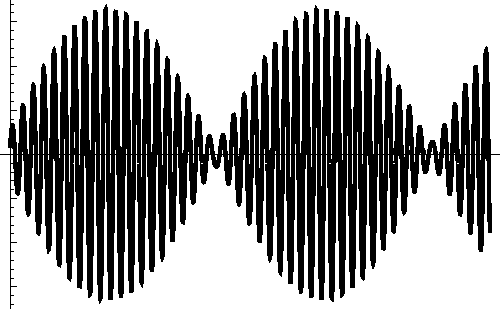
\includegraphics[width=\marginparwidth]{support/resonnance}
\\
Notice the beats. In this example, $\omega = 2$, $m=1.1$, $c\approx 0$, and $k=4$.  Since $\omega_0=\sqrt{4/1.1}\approx 2=\omega$, the solution results in large periodic oscillations. If the oscillations are too large, they will destroy the system.
}}%
Let's attach a mass-spring system to a wheel. Suppose $m=1$ and $k=4$ (with no dashpot). 
The driving force, $r(t)$, is periodic. 
\begin{enumerate}
 \item Assume the driving force is $r(t) = 7\sin(5t)$. Solve the IVP $y''+4y=7\sin(5t)$, where $y(0)=0$ and $y'(0)=0$. 
 \item
Assume $m$ and $k$ are known constants, and the driving force is $r(t) = F\sin(\omega t)$, where $\omega\neq \sqrt{k/m}$. Solve the IVP $my''+ky=F\sin(\omega t)$, where $y(0)=0$ and $y'(0)=0$.
\end{enumerate}
\end{problem}


\begin{problem}
\marginpar{{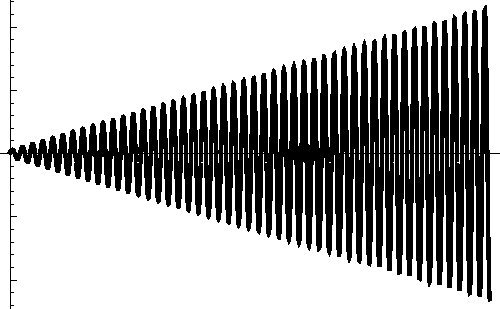
\includegraphics[width=\marginparwidth]{support/growing-oscillation}
\\
When $\omega_0=\omega$ and friction is negligible, a system will oscillate with an amplitude that grows without bound. Beware of this situation, as any mechanical system which undergoes this kind of oscillation will self destruct. 
}}%
Again, let's attach a mass-spring system to a wheel. Suppose $m=1$ and $k=4$ (with no dashpot). 
The driving force, $r(t)$, is periodic. 
\begin{enumerate}
 \item Assume the driving force is $r(t) =7 \sin(2t)$. Solve the IVP $y''+4y=7\sin(2t)$, where $y(0)=0$ and $y'(0)=0$. 
 \item Assume $m$ and $k$ are now some constant, and the driving force is $r(t) = A\sin(\omega t)$, where $\omega = \sqrt{k/m}$. Solve the IVP $my''+ky=F\sin(\omega t)$, where $y(0)=0$ and $y'(0)=0$.
\end{enumerate}
\end{problem}

Make sure you ask me in class to graph your two solutions above in Mathematica. The plots get interesting when $\omega\approx \sqrt{k/m}$, and the solution produces steady beats. You should see a rhythmic rise and fall in the amplitude of the solution.  When $\omega =  \sqrt{k/m}$, the solution grows without bound. The following YouTube videos show the collapse of the Tacoma Narrows bridge, and airplane flutter. The points to these videos is to show you the dangerous things that can (and do) happen to a structure when the designer forgets to take into account how external driving forces might interact with the internal frequencies of the mechanical system.
\begin{itemize}
 \item \href{http://www.youtube.com/watch?v=xox9BVSu7Ok}{The Tacoma Narrows bridge collapses.}
 \item \href{http://www.youtube.com/watch?v=iTFZNrTYp3k}{The tail of a small airplane begins to flutter.}
 \item \href{http://www.youtube.com/watch?v=OhwLojNerMU}{Watch a collection of flutter examples.}
 \item \href{http://www.youtube.com/watch?v=lczhD2nUedY}{An RC airplane looses its wing midflight.}
\end{itemize}

In both problems above, we assumed there was no friction ($c=0$).  Can we produce beats or resonance when there is friction? Let's analyze this problem and show that YES, bad things can still happen when friction is involved. To discover when disaster might occur, we have to work with symbolic answers and then ask, ``What would it take to produce large oscillations?''  Let's analyze this first with some specific numbers (to notice patterns) and then we'll analyze what happens symbolically.
\begin{problem}
Consider the ODE $y''+2y'+5y=5\sin(3 t)$.
\begin{enumerate}
 \item Find a general solution to this ODE.  
\WA{http://www.wolframalpha.com/input/?i=y\%27\%27\%2B2y\%27\%2B5y\%3D5\%5Csin\%283+t\%29}
 \item As $t$ increases, what happens to the homogeneous solution?
 \item If $y(0)=0$ and $y'(0)=0$, solve the IVP.
\end{enumerate}
\end{problem}

When friction enters a mass spring system, the homogeneous solution will always die out over time. The particular solution $y_p$ is called the ``steady-state'', or ``steady periodic'' solution. As time moves on, friction will damp out all oscillation except for the steady-state solution, $y_p$.  

\begin{problem}
Consider the ODE $my''+cy'+ky=F\sin(\omega t)$.
\begin{enumerate}
 \item What are the roots of the characteristic polynomial?
 \item We guess the steady-state solution (particular solution) is $y_p=A\cos(\omega t)+B\sin(\omega t)$.  Why do we never have to multiply the guess by $t$?
 \item Find the steady-state solution. As a hint, you'll probably find Cramer's Rule useful when solving for $A$ and $B$ (because you'll get a linear system with variables as coefficients). 
\WA{http://www.wolframalpha.com/input/?i=m+y\%27\%27\%28t\%29\%2Bc+y\%27\%28t\%29\%2Bk+y\%28t\%29\%3DF+\%5Csin\%28w+t\%29}
\end{enumerate}
 In class, we'll examine what it would take to get a really large amplitude for the steady-state solution (thus destroying the mechanical system).
\end{problem}
  

\subsection{Electric circuits} 
Remember that Kirchoff's voltage law states that the voltage (electromotive force) impressed on a closed loop is equal to the sum of the voltage drops across the other elements of the loop. We've summarized this by saying ``voltage in equals voltage out.'' Because we've been using complex numbers in our work, we'll use $I(t)$ to represent the current in a loop instead of $i(t)$. We've already used Kirchoff's voltage law in connection with resistors. Let's now add an inductor and a capacitor to a single loop. Each element (resistor, inductor, capacitor) produces the voltage drop given in the table below.
\begin{center}
\begin{tabular}{|l|l|l|}
\hline
Component & Voltage drop & Other\\\hline
Resistor & $RI$ & Ohm's law, where $R$ is in ohms\\\hline
Inductor & $LI' = L(dI/dt)$ & $L$ is in henrys\\\hline
Capacitor& $\dfrac{Q}{C} = \frac{1}{C}\frac{dI}{dt}$ & $Q$ is in coulombs, $C$ in farads.\\\hline
\end{tabular}
\end{center}
The charge $Q$ on a capacitor is related to the current by $I(t)=\frac{dQ}{dt}$, or $Q=\int I(t) dt$. 

We'll be studying $RC$, $RLC$, and $RL$ circuits in the next few chapters.  Table \ref{circuit table} shows the differential equations corresponding to each type of circuit.


\begin{table}[h]
\begin{center}
\begin{tabular}{ccc}
\renewcommand{\myscale}{.3}
\begin{tikzpicture}[scale=\myscale,inner sep=1pt]
%\draw[help lines,step=1cm] (0,0) grid (12,6);

%Source - like a battery
\node[label=right:$E$] at (0,3) 
{{\begin{tikzpicture}[scale=\myscale]
%	\useasboundingbox (-.5,-3) rectangle (.5,3);
	\draw (0,0) circle (1cm);
	\draw (.3,.5) -- (-.3,.5);
	\draw (0,.2) -- (0,.8);
	\draw (.3,-.5) -- (-.3,-.5);
	\draw (0,1) -- (0,3);
	\draw (0,-1) -- (0,-3);
	\end{tikzpicture}
}};

%Resistor
\node[label=right:$R$] at (6,3) 
{{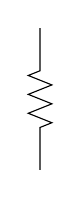
\begin{tikzpicture}[scale=\myscale]
%	\useasboundingbox (0,-3) rectangle (0,3);
	\draw (0,-3) -- ++(0,1.8) -- ++(.5,.2) 
		-- ++(-1,.4) -- ++(1,.4)
		-- ++(-1,.4) -- ++(1,.4)
		-- ++(-1,.4) -- ++(.5,.2)
		-- ++(0,1.8) ;
	\end{tikzpicture}
}};

%Straight Path
%\node at (3,6) 
%{{\begin{tikzpicture}[scale=\myscale,rotate=90]
%	\draw (0,-3) -- (0,3);
%	\end{tikzpicture}
%}};

%Arrow to represent Current
\node[label=right:$i$] at (0,5) 
{{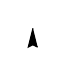
\begin{tikzpicture}[scale=\myscale,rotate=0]
	\filldraw (0,.4) -- (-.2,-.4) -- (0,-.3) -- (.2,-.4);
	\end{tikzpicture}
}};

%Loops
\node[label=above:$L$] at (3,6) 
{{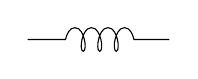
\begin{tikzpicture}[scale=\myscale,rotate=90]
	\useasboundingbox (-.5,-3) rectangle (.5,3);
	\draw (0,-3) -- ++(0,1.5) 
	.. controls+(15:.2) and +(-90:.25) .. ++(.5,.4) 
	.. controls+(90:.25) and +(-15:.2) .. ++(-.5,.4) 
	.. controls+(-15:-.2) and +(90:.1) .. ++(-.5,-.05) 
	.. controls+(-90:.1) and +(15:-.2) .. ++(.5,-.05) 
	.. controls+(15:.2) and +(-90:.25) .. ++(.5,.4) 
	.. controls+(90:.25) and +(-15:.2) .. ++(-.5,.4) 
	.. controls+(-15:-.2) and +(90:.1) .. ++(-.5,-.05) 
	.. controls+(-90:.1) and +(15:-.2) .. ++(.5,-.05) 
	.. controls+(15:.2) and +(-90:.25) .. ++(.5,.4) 
	.. controls+(90:.25) and +(-15:.2) .. ++(-.5,.4) 
	.. controls+(-15:-.2) and +(90:.1) .. ++(-.5,-.05) 
	.. controls+(-90:.1) and +(15:-.2) .. ++(.5,-.05) 
	.. controls+(15:.2) and +(-90:.25) .. ++(.5,.4) 
	.. controls+(90:.25) and +(-15:.2) .. ++(-.5,.4) 
	-- (0,3);
	\end{tikzpicture}
}};


%Capacitor
\node[label=above:$C$] at (3,0) 
{{\begin{tikzpicture}[scale=\myscale,rotate=90]
%	\useasboundingbox (0,-3) rectangle (0,3);
	\draw (0,-3) -- ++(0,2.8) 
		-- ++(.5,0) -- ++(-1,0) 
		++(0,.4) -- ++(1,0)
		-- ++(-.5,0) -- ++(0,2.8);
	\end{tikzpicture}
}};


\end{tikzpicture}

&
\renewcommand{\myscale}{.3}
\begin{tikzpicture}[scale=\myscale,inner sep=1pt]
%\draw[help lines,step=1cm] (0,0) grid (12,6);

%Source - like a battery
\node[label=right:$E$] at (0,3) 
{{\begin{tikzpicture}[scale=\myscale]
%	\useasboundingbox (-.5,-3) rectangle (.5,3);
	\draw (0,0) circle (1cm);
	\draw (.3,.5) -- (-.3,.5);
	\draw (0,.2) -- (0,.8);
	\draw (.3,-.5) -- (-.3,-.5);
	\draw (0,1) -- (0,3);
	\draw (0,-1) -- (0,-3);
	\end{tikzpicture}
}};

%Resistor
\node[label=right:$R$] at (6,3) 
{{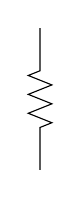
\begin{tikzpicture}[scale=\myscale]
%	\useasboundingbox (0,-3) rectangle (0,3);
	\draw (0,-3) -- ++(0,1.8) -- ++(.5,.2) 
		-- ++(-1,.4) -- ++(1,.4)
		-- ++(-1,.4) -- ++(1,.4)
		-- ++(-1,.4) -- ++(.5,.2)
		-- ++(0,1.8) ;
	\end{tikzpicture}
}};

%Straight Path
\node at (3,6) 
{{\begin{tikzpicture}[scale=\myscale,rotate=90]
	\draw (0,-3) -- (0,3);
	\end{tikzpicture}
}};

%Arrow to represent Current
\node[label=above:$i$] at (3,6) 
{{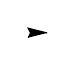
\begin{tikzpicture}[scale=\myscale,rotate=-90]
	\filldraw (0,.4) -- (-.2,-.4) -- (0,-.3) -- (.2,-.4);
	\end{tikzpicture}
}};

%Inductor
%\node[label=above:$L$] at (3,6) 
%{{\begin{tikzpicture}[scale=\myscale,rotate=90]
%	\useasboundingbox (-.5,-3) rectangle (.5,3);
%	\draw (0,-3) -- ++(0,1.5) 
%	.. controls+(15:.2) and +(-90:.25) .. ++(.5,.4) 
%	.. controls+(90:.25) and +(-15:.2) .. ++(-.5,.4) 
%	.. controls+(-15:-.2) and +(90:.1) .. ++(-.5,-.05) 
%	.. controls+(-90:.1) and +(15:-.2) .. ++(.5,-.05) 
%	.. controls+(15:.2) and +(-90:.25) .. ++(.5,.4) 
%	.. controls+(90:.25) and +(-15:.2) .. ++(-.5,.4) 
%	.. controls+(-15:-.2) and +(90:.1) .. ++(-.5,-.05) 
%	.. controls+(-90:.1) and +(15:-.2) .. ++(.5,-.05) 
%	.. controls+(15:.2) and +(-90:.25) .. ++(.5,.4) 
%	.. controls+(90:.25) and +(-15:.2) .. ++(-.5,.4) 
%	.. controls+(-15:-.2) and +(90:.1) .. ++(-.5,-.05) 
%	.. controls+(-90:.1) and +(15:-.2) .. ++(.5,-.05) 
%	.. controls+(15:.2) and +(-90:.25) .. ++(.5,.4) 
%	.. controls+(90:.25) and +(-15:.2) .. ++(-.5,.4) 
%	-- (0,3);
%	\end{tikzpicture}
%}};


%Capacitor
\node[label=above:$C$] at (3,0) 
{{\begin{tikzpicture}[scale=\myscale,rotate=90]
%	\useasboundingbox (0,-3) rectangle (0,3);
	\draw (0,-3) -- ++(0,2.8) 
		-- ++(.5,0) -- ++(-1,0) 
		++(0,.4) -- ++(1,0)
		-- ++(-.5,0) -- ++(0,2.8);
	\end{tikzpicture}
}};


\end{tikzpicture}

& 
\renewcommand{\myscale}{.3}
\begin{tikzpicture}[scale=\myscale,inner sep=1pt]
%\draw[help lines,step=1cm] (0,0) grid (12,6);

%Source - like a battery
\node[label=right:$E$] at (0,3) 
{{\begin{tikzpicture}[scale=\myscale]
%	\useasboundingbox (-.5,-3) rectangle (.5,3);
	\draw (0,0) circle (1cm);
	\draw (.3,.5) -- (-.3,.5);
	\draw (0,.2) -- (0,.8);
	\draw (.3,-.5) -- (-.3,-.5);
	\draw (0,1) -- (0,3);
	\draw (0,-1) -- (0,-3);
	\end{tikzpicture}
}};

%Resistor
\node[label=right:$R$] at (6,3) 
{{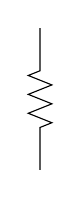
\begin{tikzpicture}[scale=\myscale]
%	\useasboundingbox (0,-3) rectangle (0,3);
	\draw (0,-3) -- ++(0,1.8) -- ++(.5,.2) 
		-- ++(-1,.4) -- ++(1,.4)
		-- ++(-1,.4) -- ++(1,.4)
		-- ++(-1,.4) -- ++(.5,.2)
		-- ++(0,1.8) ;
	\end{tikzpicture}
}};

%Straight Path
\node at (3,0) 
{{\begin{tikzpicture}[scale=\myscale,rotate=90]
	\draw (0,-3) -- (0,3);
	\end{tikzpicture}
}};

%Arrow to represent Current
\node[label=above:$i$] at (3,0) 
{{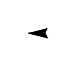
\begin{tikzpicture}[scale=\myscale,rotate=90]
	\filldraw (0,.4) -- (-.2,-.4) -- (0,-.3) -- (.2,-.4);
	\end{tikzpicture}
}};

%Inductor
\node[label=above:$L$] at (3,6) 
{{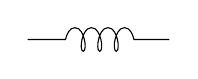
\begin{tikzpicture}[scale=\myscale,rotate=90]
	\useasboundingbox (-.5,-3) rectangle (.5,3);
	\draw (0,-3) -- ++(0,1.5) 
	.. controls+(15:.2) and +(-90:.25) .. ++(.5,.4) 
	.. controls+(90:.25) and +(-15:.2) .. ++(-.5,.4) 
	.. controls+(-15:-.2) and +(90:.1) .. ++(-.5,-.05) 
	.. controls+(-90:.1) and +(15:-.2) .. ++(.5,-.05) 
	.. controls+(15:.2) and +(-90:.25) .. ++(.5,.4) 
	.. controls+(90:.25) and +(-15:.2) .. ++(-.5,.4) 
	.. controls+(-15:-.2) and +(90:.1) .. ++(-.5,-.05) 
	.. controls+(-90:.1) and +(15:-.2) .. ++(.5,-.05) 
	.. controls+(15:.2) and +(-90:.25) .. ++(.5,.4) 
	.. controls+(90:.25) and +(-15:.2) .. ++(-.5,.4) 
	.. controls+(-15:-.2) and +(90:.1) .. ++(-.5,-.05) 
	.. controls+(-90:.1) and +(15:-.2) .. ++(.5,-.05) 
	.. controls+(15:.2) and +(-90:.25) .. ++(.5,.4) 
	.. controls+(90:.25) and +(-15:.2) .. ++(-.5,.4) 
	-- (0,3);
	\end{tikzpicture}
}};


%Capacitor
%\node[label=above:$C$] at (3,0) 
%{{\begin{tikzpicture}[scale=\myscale,rotate=90]
%	\draw (0,-3) -- ++(0,2.8) 
%		-- ++(.5,0) -- ++(-1,0) 
%		++(0,.4) -- ++(1,0)
%		-- ++(-.5,0) -- ++(0,2.8)
%	\end{tikzpicture}
%}};


\end{tikzpicture}

\\
An $RLC$-circuit
&An $RC$-circuit
&An $RL$-circuit
\\\hline
$L I'+ RI+ \frac{1}{C}\int I(t) dt = E(t)$
&$RI+ \frac{1}{C}\int I(t) dt = E(t)$
&$L I'+ RI = E(t)$
\\
$L Q''+ RQ'+ \frac{1}{C}Q = E(t)$
&$RQ'+ \frac{1}{C}Q = E(t)$
&%$L Q''+ RQ' = E(t)$
\\
$L I''+ RI'+ \frac{1}{C}I = E'(t)$
&$RI'+ \frac{1}{C}I = E'(t)$
&%$L I''+ RI' = E'(t)$
\\\hline
\end{tabular}
\end{center}
\caption{Typical diagrams of $RCL$, $RC$, and $RL$ circuits, and their corresponding ODEs. The first row is an integro-differential equation for the current $I(t)$. The second row is the ODE for the charge $Q$ on the capacitor. The third row is the derivative of the first row. \label{circuit table}
}
\end{table}

In a circuit  with one resistor, one inductor, and one capacitor (an $RLC$ circuit), if the electromotive force is $E(t)$, then Kirchoff's Voltage law gives the integro-differential equation 
$$L I'+ RI+ \frac{1}{C}Q(t) =E(t) \quad \text{or}\quad L I'+ RI+ \frac{1}{C}\int I(t) dt = E(t).$$  
Differentiating both sides removes the integral and gives
$$L I''+ RI'+ \frac{1}{C}I(t) = E'(t),$$ which is a second order linear differential equation with constant coefficients. However, the initial conditions are in terms of initial charge $Q(0)$ and initial current $I(0)$. To solve the differential equation for $I$, we need $I'(0)$, which we can get from the equation $ L I'(t)+ RI(t)+ \frac{1}{C}Q(t) =E(t)$. Problem 14.13 in Schaum's provides an excellent example that summarizes the solution technique.
 
\begin{problem}
Consider an $RLC$ circuit with $L=1/2$, $R=2$, and $C=2/3$. Let's plug the circuit into an alternating current power source (like a wall outlet), which means we might have something like $E(t) = 2\cos(3t)$.  Initially, assume that the current is zero and the charge on the capacitor is zero. We'd like to find the current at any time $t$ in the circuit.
\begin{enumerate}
 \item Explain why the current satisfies $I''+4I'+3I=-12\sin(3t)$. Find a general solution to this ODE.
\WA{http://www.wolframalpha.com/input/?i=y\%27\%27\%2B4y\%27\%2B3y\%3D-12\%5Csin\%283t\%29}
 \item We know that $I(0)=0$ and $Q(0)=0$.  Use the equation $L I'(t)+ RI(t)+ \frac{1}{C}Q(t) =E(t)$ to explain why $I'(0) = 4$. 
 \item Find the current in the wire at any time $t$ by solving the corresponding IVP. Use the initial conditions you found in the previous part.
\WA{http://www.wolframalpha.com/input/?i=y\%27\%27\%2B4y\%27\%2B3y\%3D-12\%5Csin\%283t\%29\%2C+y\%280\%29\%3D0\%2C+y\%27\%280\%29\%3D4}
 \item What is the steady-state current? (Which part of your solution above does not vanish after sufficient time has passed? This would be the current flowing through the circuit after the initial conditions have died out.)
\end{enumerate}
\end{problem}

\begin{problem}
Consider an $RLC$ circuit with $L=1$, $R=8$, and $C=\frac{1}{25}$. Let's plug the circuit into a 12 V battery, so we have $E(t) =12$.  Initially, assume that the current is zero and the charge on the capacitor is zero. We'd like to find the current at any time $t$ in the circuit.
\begin{enumerate}
 \item State the IVP whose solution would give the current at any time $t$. (What's the ODE, and what are the initial conditions $I(0)$ and $I'(0)$).  [Hint: Use the equation $L I'(t)+ RI(t)+ \frac{1}{C}Q(t) =E(t)$ to find $I'(0)$.] 
 \item Find the current in the wire at any time $t$. Check your answer with WolframAlpha (you'll want to use $y$ instead of $I$).
 \item What's the steady-state current?
\end{enumerate}

\end{problem}

\begin{observation}
Mechanical models are expensive to build.  Electrical models are fairly simple to build and measure.  If you need to create a mechanical system, it may prove beneficial financially to start with an electrical model. Engineers spend another semester on this idea in system dynamics.  Hydraulic systems are also very closely related. In bridging between mechanical and electrical systems, we compare the following variables. 
\begin{center}
\begin{tabular}{|c|c|c|c|c|c|}
\hline
Mechanical System&$m$&$c$&$k$&$r(t)=F_0\cos\omega t$&$y(t)$\\\hline
Electrical System&$L$&$R$&$1/C$&$E'(t) = E_0\omega\cos\omega t$&$I(t)$\\
\hline
\end{tabular}
\end{center}
Solving a problem in one system (either mechanical or electrical) can provide useful results in the other.  
\end{observation}



\section*{Wrap up}
\addcontentsline{toc}{section}{Wrap Up}

This concludes the chapter.  Look at the objectives at the beginning of the chapter. Can you now do all the things you were promised? 


\begin{problem}[Lesson Plan Creation] \marginpar{This counts as 4 prep problems. My hope is that you spend at least an hour creating your one-page lesson plan.}
Your assignment: organize what you've learned into a small collection of examples that illustrates the key concepts. I'll call this your one-page lesson plan. You may use both sides. The objectives at the beginning of the chapter give you a list of the key concepts. Once you finish your lesson plan, scan it into a PDF document (use any scanner on campus), and then upload the document to I-Learn.
\end{problem}





